\documentclass[12pt,letterpaper]{article}
\usepackage[utf8]{inputenc}
\usepackage{amsmath}
\usepackage{amsfonts}
\usepackage{amssymb}
\usepackage{graphicx}
\usepackage{fancybox}
\usepackage{caption}
\usepackage{listings}
\usepackage{hyperref}
\setlength{\captionmargin}{10mm}
\renewcommand\captionfont{\it}
\renewcommand\captionlabelfont{\bf}
\hypersetup{
   pdfauthor = {Kim Siang Khaw},
	colorlinks=true, citecolor=blue, linkcolor=blue, bookmarksnumbered = true,
}
\usepackage[left=2.0cm,right=2.0cm,top=2cm,bottom=2cm]{geometry}
\author{Kim Siang Khaw \\
University of Washington}
\title{\textbf{SLAC 2016 data analysis: Documentation and explanations}}

\begin{document}
\maketitle

\section{Introduction}
Prerequisites for this tutorial are a basic understanding of what the Muon g-2 experiment and PbF$_2$ calorimeters~\cite{Fienberg2015} are, some knowledge about the electromagnetic (EM) shower and the ROOT data analysis framework~\cite{ROOT}. You can follow the exercise sheet step by step which guides you to the data analysis using the reconstructed electron EM shower clusters. Some analyses may require the use of reconstructed crystal hit, which is the basic object of forming a cluster. Advanced users are encouraged to use the FNAL's \textit{art} framework for the data analysis.
%
%trim left bottom right top
\begin{figure}[htbp]
\centering
%\fbox{\includegraphics[trim=0cm 5.5cm 0cm 5.5cm ,width=0.9\textwidth]{pics/EMShower}} guide line for trimming
\includegraphics[trim=3cm 1cm 3cm 0cm, width=0.4\textwidth]{pics/EMShower}
\caption{Illustration of the electromagnetic shower of an electron injected from the left to the right, in a $9\times6$ array PbF$_2$ calorimeter. Cherenkov lights created by the charged shower particles are collected by the Silicon Photomultipliers (SiPMs) glued to the end of the PbF$_2$ crystals.}
\end{figure}

Data analysis of this test beam has several components that are common with the Muon g-2 experiment data analysis framework~\cite{Khaw2016}. The physics objects that will be used for most of the analyses are the crystal hits and the hit clusters.
These objects are reconstructed from the digitized waveform, after going through steps like pulsing fitting, energy calibration, gain correction, time correction and hit clustering. During the first week of the test beam, all these reconstruction steps
will be refined based on the data taken and these will be taken care of by those who are familiar with the \textit{art} framework. The main focus of this documentation is on the physics analysis using high level physics objects like the crystal hit and the cluster, using a C++/ROOT standalone framework. The user can proceed to more sophisticated analysis once he/she is familiar with the tools. The standalone framework can also be used as a stepping stone to develop analysis algorithm before migrating it to the \textit{art} framework.

Several studies that will be covered for the data analysis (non-exhaustive list) are
\begin{itemize}
\item energy resolution of the calorimeter
\item position and angular resolution of the calorimeter
\item degeneracy of the position and angular information of the calorimeter
\item stability of gain monitoring system
\item pile up separation for multi-electron events
\end{itemize}

Further information about how the data will be processed and analyzed are summarized in Appendix A (to be updated).

%% For myself
%% Explain the offline data analysis flow here

\section{Data samples}
This section explains the naming and the locations of the data files (Local location will be obsolete once we move everything
to the PNFS disk at FNAL).

\subsection{File naming}

All the created art/ROOT and ROOT files will have the same run number as the MIDAS they are extracted from.

\begin{table}[htbp]
\centering
\caption{Data samples and descriptions. The ROOT full data includes raw waveforms, chopped islands and processed data like fit results and crystal hits. The ROOT analysis data has only processed data.}
\begin{tabular}{|c|c|} \hline 
filename & type \\ \hline 
gm2slac\_run0xxxx.art & data ready for art-based analysis \\ \hline 
gm2slac\_run0xxxx\_raw.root & full data for standalone C++ analysis \\ \hline 
gm2slac\_run0xxxx.root & analysis data for standalone C++ analysis \\ \hline 
\end{tabular} \label{tab:datasamples}
\end{table}

\subsection{Location of the files}

For the following steps, you have to be connected to the local Wifi network \verb+T536-local+.
All the art/ROOT and ROOT files are stored in the $2\times3$TB HDD in the \verb+g2analysis+ machine.
Use the following command to copy over the data files that you want to analyze: 
%
\begin{lstlisting}[frame=single, basicstyle=\ttfamily\footnotesize]
scp -r g2muon@g2analysis:/data1/slac2016/analysis/gm2slac_run0xxxx.root . 
scp -r g2muon@g2analysis:/data2/slac2016/art/gm2slac_run0xxxx.art .
\end{lstlisting}
%
Or you can use \verb+rsync+ if you have enough space in your hard drive:
%
\begin{lstlisting}[frame=single, basicstyle=\ttfamily\footnotesize]
rsync -avurt g2muon@g2analysis:/data1/slac2016/analysis/ YOUR_LOCAL_DISK/
rsync -avurt g2muon@g2analysis:/data2/slac2016/art/ YOUR_LOCAL_DISK/
\end{lstlisting}
%
Or a better way is to use \verb+sshfs+ to mount the disk onto your laptop:
\begin{lstlisting}[frame=single, basicstyle=\ttfamily\footnotesize]
sshfs g2muon@g2analysis:/data1/slac2016/analysis YOUR_LOCAL_DISK
sshfs g2muon@g2analysis:/data2/slac2016/art YOUR_LOCAL_DISK
\end{lstlisting}

\section{Data format and structure for the ROOT tree}
The data samples for this tutorial are stored in ROOT trees. The tree contains a collection of variables (called branches) which are filled once per event (could be 1 or more electrons). The list of variables along with their data type and further explanations are given in the following.

\subsection*{For studies using higher level objects}

\begin{itemize}

\item \verb+FitResult_EventNum+ (\verb+vector<int>+): event number of this fit result
\item \verb+FitResult_CaloNum+ (\verb+vector<int>+): calorimeter number of this fit result
\item \verb+FitResult_XtalNum+ (\verb+vector<int>+): crystal number of this fit result
\item \verb+FitResult_IslandNum+ (\verb+vector<int>+): island number of this fit result
\item \verb+FitResult_UtcaSlotNum+ (\verb+vector<int>+): utca slot number of this fit result
\item \verb+FitResult_ChannelNum+ (\verb+vector<int>+): rider channel number of this fit result
\item \verb+FitResult_Energy+ (\verb+vector<double>+): energy (number of photons) of this fit result
\item \verb+FitResult_Time+ (\verb+vector<double>+): time (clock tick of 800 MHz) of this fit result within the fill/event
\item \verb+FitResult_Pedestal+ (\verb+vector<double>+): pedestal of this fit result
\item \verb+FitResult_Chi2+ (\verb+vector<double>+): Chi squared of this fit result
\item \verb+FitResult_ClockCounter+ (\verb+vector<long long>+): time stamp (clock tick of 40 MHz) of this fit result from Rider header information

\item \verb+XtalHit_EventNum+ (\verb+vector<int>+): event number of this crystal hit
\item \verb+XtalHit_CaloNum+ (\verb+vector<int>+): calorimeter number of this crystal hit
\item \verb+XtalHit_XtalNum+ (\verb+vector<int>+): crystal number of this crystal hit
\item \verb+XtalHit_IslandNum+ (\verb+vector<int>+): island number of this crystal hit
\item \verb+XtalHit_UtcaSlotNum+ (\verb+vector<int>+): utca slot number of this crystal hit
\item \verb+XtalHit_ChannelNum+ (\verb+vector<int>+): rider channel number of this crystal hit
\item \verb+XtalHit_Energy+ (\verb+vector<double>+): energy (number of photons) of this crystal hit
\item \verb+XtalHit_Time+ (\verb+vector<double>+): time (clock tick of 800 MHz) of this crystal hit within the fill/event
\item \verb+XtalHit_ClockCounter+ (\verb+vector<long long>+): time stamp (clock tick of 40 MHz) of this crystal hit from Rider header information

\item \verb+Cluster_EventNum+ (\verb+vector<int>+): event number of this cluster 
\item \verb+Cluster_CaloNum+ (\verb+vector<int>+): calorimeter number of this cluster
\item \verb+Cluster_IslandNum+ (\verb+vector<int>+): island number of this cluster
\item \verb+Cluster_Energy+ (\verb+vector<double>+): energy (number of photons) of this cluster
\item \verb+Cluster_Time+ (\verb+vector<double>+): time (clock tick) of this cluster 
\item \verb+Cluster_X+ (\verb+vector<double>+): local x-position of this cluster (logarithmic-weighted)
\item \verb+Cluster_Y+ (\verb+vector<double>+): local x-position of this cluster (logarithmic-weighted)

\item \verb+Italiano_EventNum+ (\verb+vector<int>+): event number of this analyzed laser crate waveform
\item \verb+Italiano_CaloNum+ (\verb+vector<int>+): calorimeter number of this analyzed laser crate waveform
\item \verb+Italiano_XtalNum+ (\verb+vector<int>+): crystal number of this analyzed laser crate waveform
\item \verb+Italiano_IslandNum+ (\verb+vector<int>+): island number of this analyzed laser crate waveform
\item \verb+Italiano_UtcaSlotNum+ (\verb+vector<int>+): utca slot number of this analyzed laser crate waveform
\item \verb+Italiano_ChannelNum+ (\verb+vector<int>+): rider channel number of this analyzed laser crate waveform
\item \verb+Italiano_Amplitude+ (\verb+vector<double>+): amplitude (ADC samples) of this analyzed laser crate waveform
\item \verb+Italiano_Time+ (\verb+vector<double>+): time (clock tick of 800 MHz) of this analyzed laser crate waveform within the fill/event
\item \verb+Italiano_Pedestal+ (\verb+vector<double>+): pedestal of this analyzed laser crate waveform
\item \verb+Italiano_Area+ (\verb+vector<double>+): Area of this analyzed laser crate waveform
\item \verb+Italiano_ClockCounter+ (\verb+vector<long long>+): time stamp (clock tick of 40 MHz) of this analyzed laser crate waveform from Rider header information
\end{itemize}

\subsection*{For studies using lower level objects}
Blow are the Tleaves of the \verb+islandTree+.

\begin{itemize}
\item \verb+RunNum+ (\verb+int+): run number of this island
\item \verb+EventNum+ (\verb+int+): event number of this island
\item \verb+FillType+ (\verb+int+): fill type of this island (1 is muon fill, 2 is laser fill)
\item \verb+TriggerNum+ (\verb+int+): trigger number of this island
\item \verb+CaloNum+ (\verb+int+): calorimeter number of this island
\item \verb+XtalNum+ (\verb+int+): crystal number of this island
\item \verb+IslandNum+ (\verb+int+): island number of this island
\item \verb+UtcaSlotNum+ (\verb+int+): utca slot number of this island
\item \verb+ChannelNum+ (\verb+int+): rider channel number of this island
\item \verb+Length+ (\verb+int+): number of sample of this island
\item \verb+Time+ (\verb+int+): time (clock tick of 800 MHz) of the first sample of this island within the fill/event
\item \verb+ClockCounter+ (\verb+long+): time stamp (clock tick of 40 MHz) of this island from Rider header information
\item \verb+Trace+ (\verb+vector<short>+): ADC samples of this island
\end{itemize}

\section{Standalone C++ Analysis framework}

The package \verb+SLAC2016Ana+ contains an example \verb+C+++ framework to help you getting started. You can get it from the github.com by \verb+git clone https://github.com/kimsiang/SLAC2016+. You can build your additional analysis code on top of this example or write a new one based on it. The example is already running but it's not doing much yet. You can compile the analysis code by first sourcing your ROOT environment (e.g. \verb+source /usr/local/bin/thisroot.sh+) and then followed by executing the command \verb+make+.

This will read the necessary ingredients for compilation from the \verb+Makefile+ in the same directory. Don't have to worry much about this file at the moment unless you want to add in more classes to the analysis code.
The point is that it creates an executable named \verb+ana+. You can then execute the program by the command \verb+./ana input.script+ where \verb+input.script+ includes a path to the root file that you want to analyze (e.g. \verb+./test.root+). 

A description of the individual components of the example are given in the following list. Indicated are also the places where you should start adding your own code:

\begin{itemize}
\item  \verb+main.cxx+: This is the first starting point. It contains the \verb+main()+ function which is necessary for any \verb+C+++ program. The first step is to create instances of \verb+MyAna()+ class which is implemented in the files \verb+MyAna.h+ and \verb+MyAna.C+ (explained in the next items). The \verb+TChain+ represents the ROOT tree discussed in section 3. The files which should be read from disk are specified in the function \verb+Add(filename)+. The tree is then read and processed by the \verb+MyAna()+ class which takes the \verb+TChain+ as argument. The real work is then done in the \verb+Loop()+ function of the \verb+MyAna()+ class which is discussed in the next two items. 

\item \verb+MyAna.h+: Definition of the class \verb+MyAna+, which inherits from the \verb+TTree::MakeClass+. It declares variables and ROOT objects that will be used or stored in your analysis. Several basic functions that are common among event-based particle physics analysis like \verb+initialize()+, \verb+clear()+, \verb+execute()+ and\verb+finalize()+ are declared here.
%% to myself
%% need to change the names like Loop, execute, etc because it is a bit confusing
\item \verb+MyAna.C+: The main function which is called automatically which processing the ROOT trees are \verb+Loop()+. The \verb+Loop()+ function is called only once per run. In the \verb+Loop()+ function, \verb+initialize()+ is called at the beginning of the analysis run, \verb+clear()+ and \verb+execute()+ is called every event, and \verb+finalize()+ at the end of the analysis run.

\item \verb+t1.h+: Header file for the class \verb+t1+ created using \verb+TTree::MakeClass+.  

\item \verb+t1.C+: Source file for the class \verb+t1+ created using \verb+TTree::MakeClass+. The class \verb+Loop()+ is used by \verb+MyAna+ to loop through each \verb+TBranch+.

\item \verb+PlotAll.C+: A ROOT macro which can be used for automatic plotting of a set of histograms which are stored in a ROOT file. Please read the header of the file on how to use it. 
\end{itemize}


\section{ROOT-based offline event display}

A ROOT-based offline event display is also developed to increase the user friendliness of the data analysis. As shown in Figure~\ref{fig:GUI}, this GUI interface allows the user to inspect the fit results of the template fit algorithm by overlaying it with the island samples.
More functionality will be added in the coming days.

\begin{figure}[htbp]
\centering
%\fbox{\includegraphics[trim=0cm 5.5cm 0cm 5.5cm ,width=0.9\textwidth]{pics/EMShower}} guide line for trimming
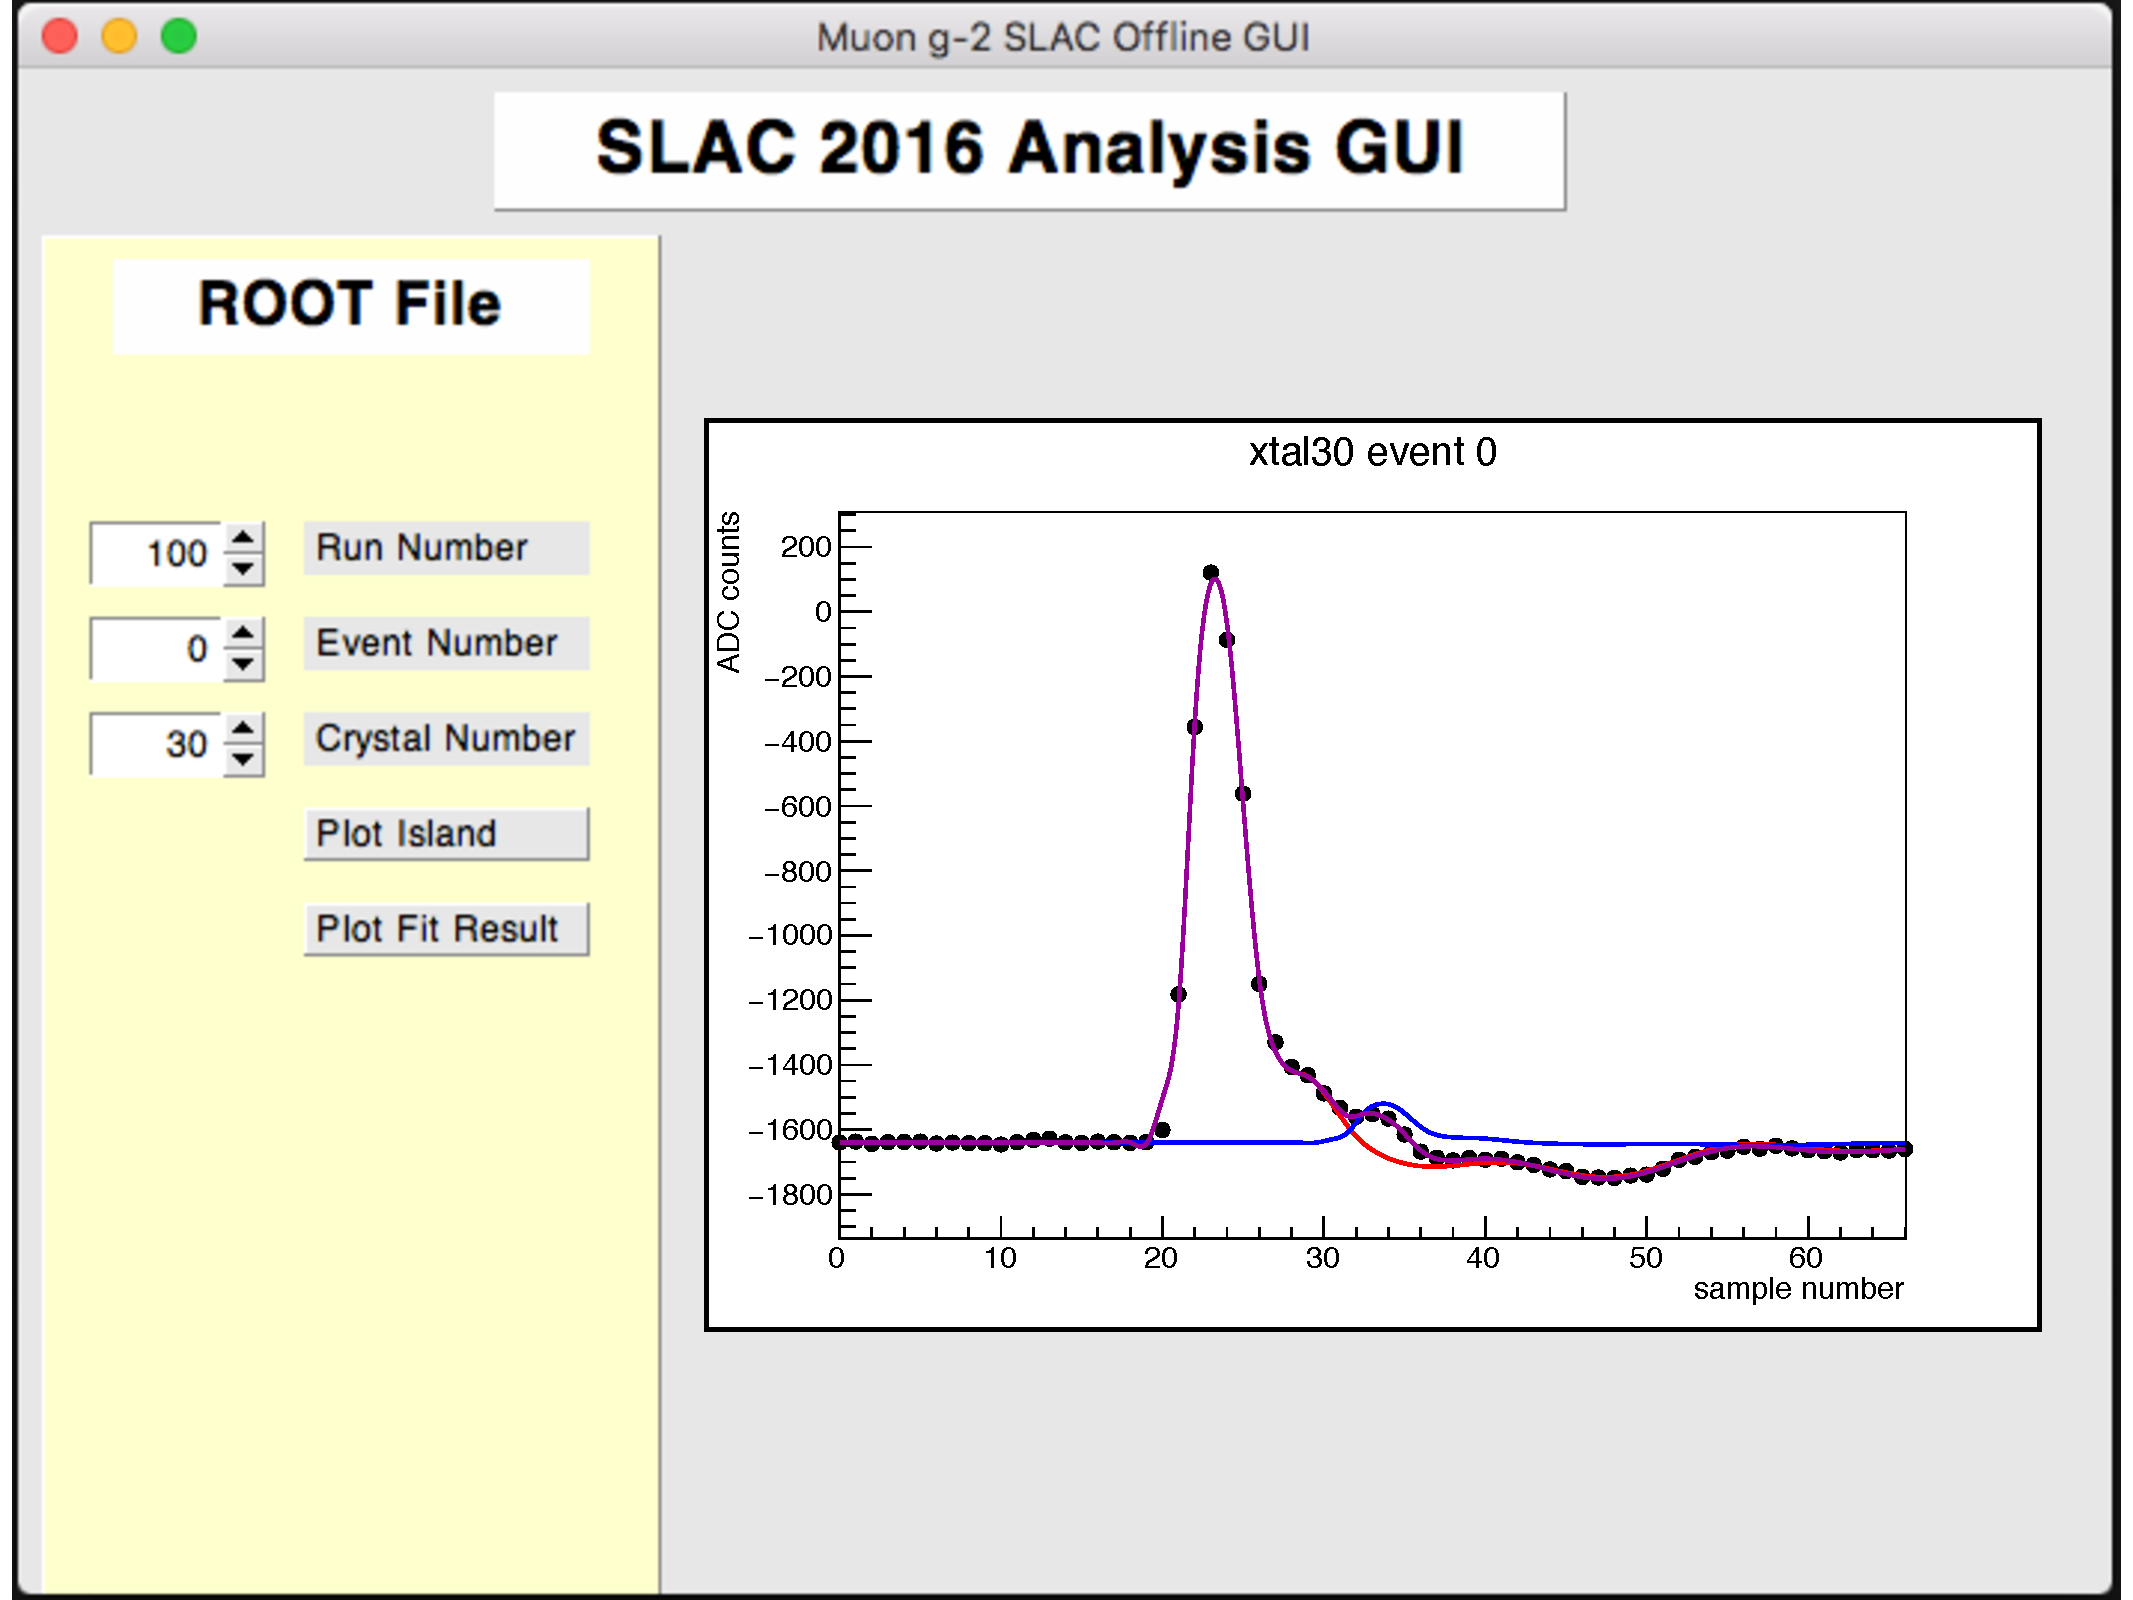
\includegraphics[width=0.75\textwidth]{pics/SLAC2016_Analysis_GUI}
\caption{SLAC Offline analysis GUI. This is a very preminary prototype.}\label{fig:GUI}
\end{figure}


\newpage
\appendix

\section{Data analysis framework}

\begin{figure}[htbp]
\centering
%\fbox{\includegraphics[trim=0cm 5.5cm 0cm 5.5cm ,width=0.9\textwidth]{pics/EMShower}} guide line for trimming
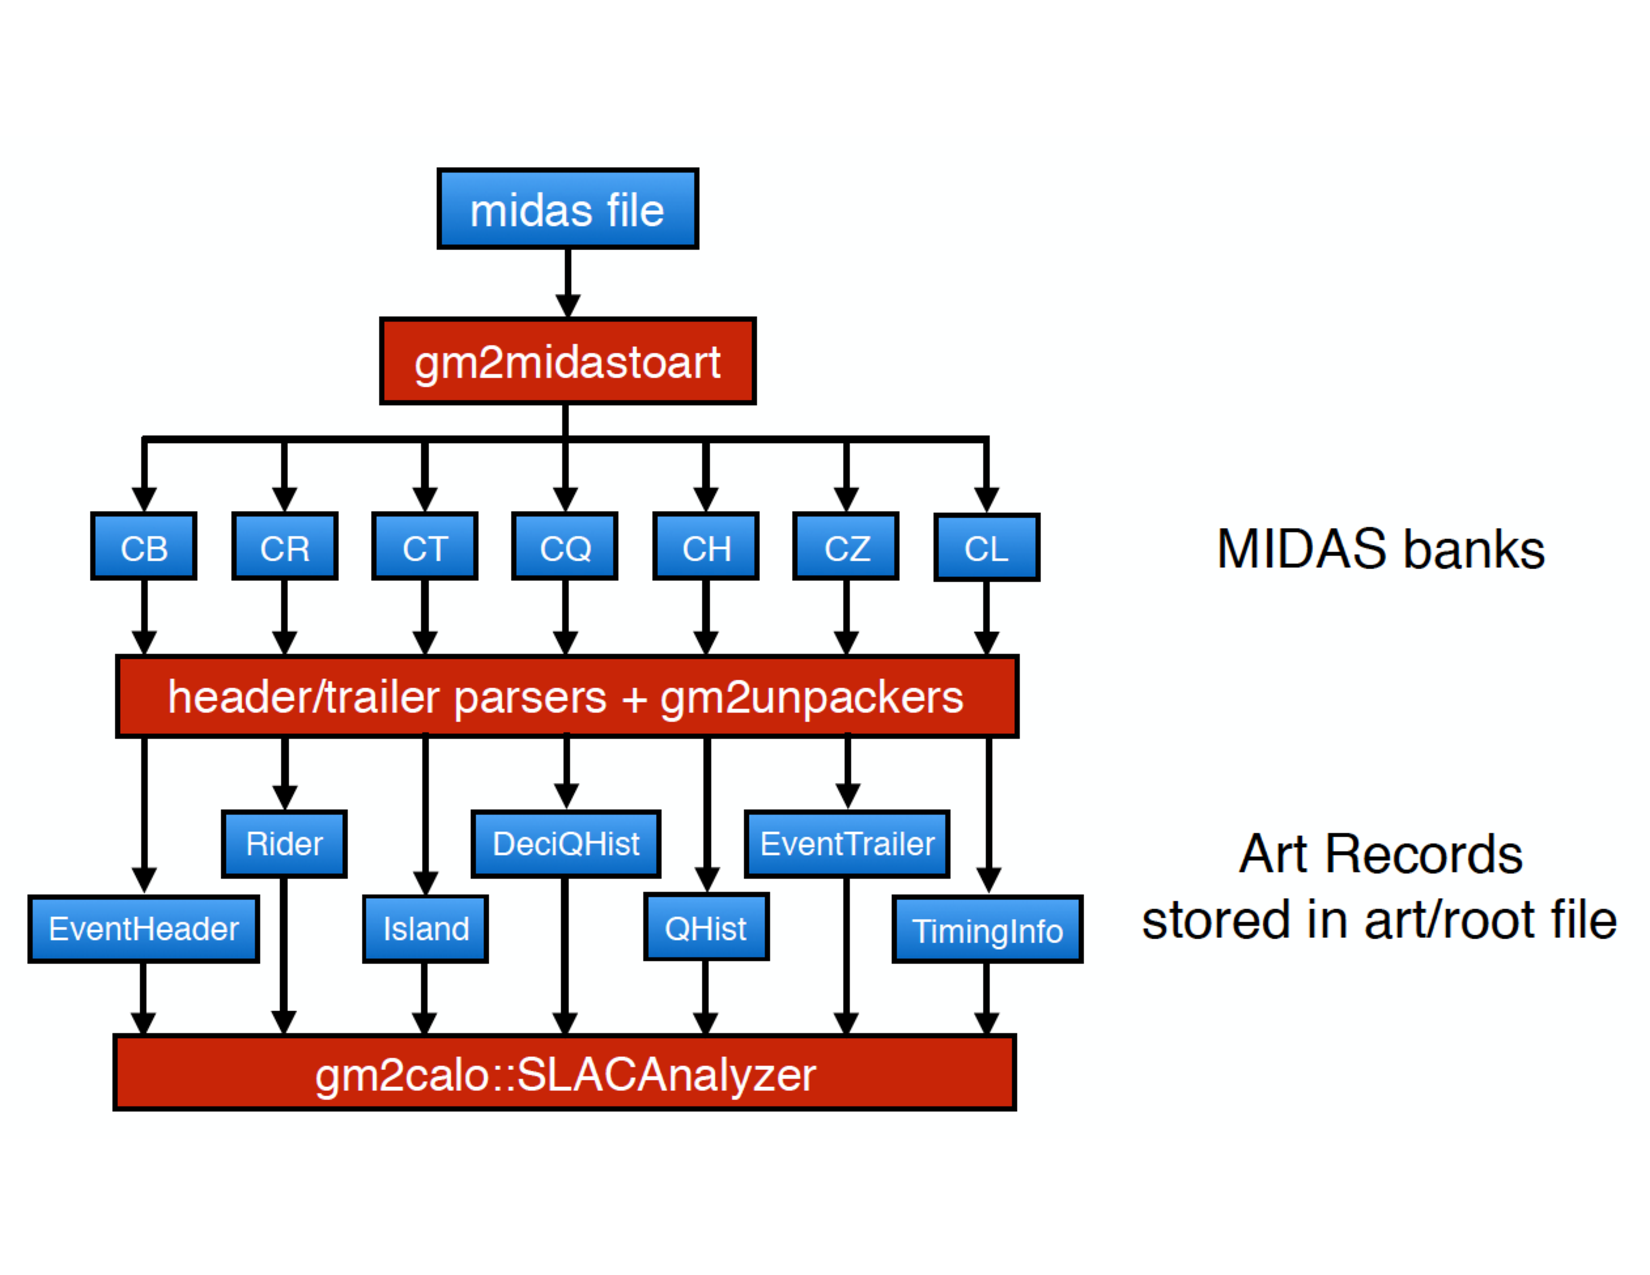
\includegraphics[width=0.8\textwidth]{pics/offline_slac_framework}
\caption{Offline framework for SLAC experimental data.}
\end{figure}

The data analysis of this test beam has several components. First we need to convert the raw data stored in a MIDAS file (\verb+.mid+ or \verb+.mid.gz+) to \textit{art} data products stored in a ROOT file.
This is handled using \textit{art} framework's modules and is doing nothing more than storing \verb+16-bit+ or \verb+32-bit+ word into \verb+vectors+. Next we unpack these \verb+vectors+
and give them contexts based on the header information stored within the \verb+vectors+. As this step, all the information are stored as data products you are probably familiar with: \verb+RiderArtRecord+,
 \verb+IslandArtRecord+, etc.

\section{Header information}
This section provides the information regarding user interface to the event, AMC13 and rider header information. All the information are stored in the art/ROOT files and standalone ROOT files with the TBranch structures in the following sections.

\section{Header and trailer formats}

This section compiles all the available header data formats. Please refer to \url{http://gm2-docdb.fnal.gov:8080/cgi-bin/ShowDocument?docid=3409} for more details.

\begin{figure}[htbp]
\centering
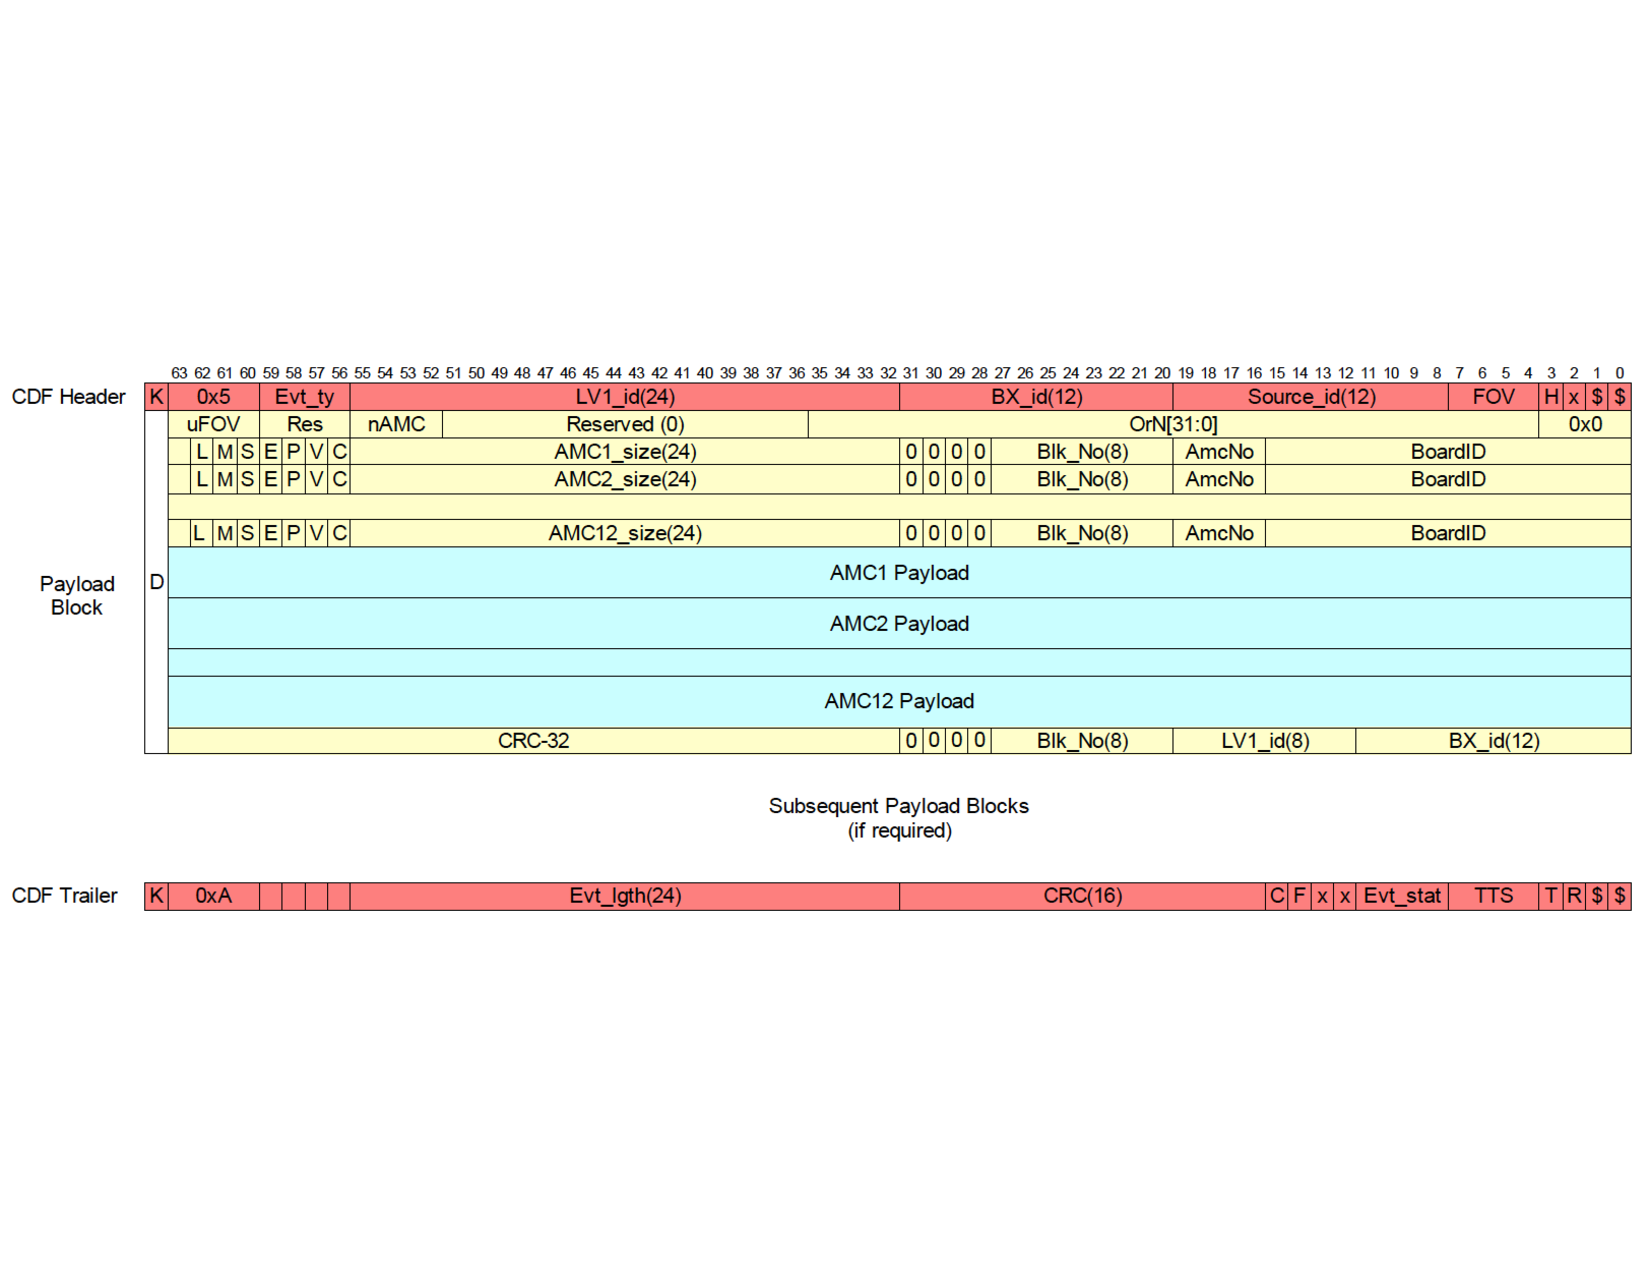
\includegraphics[trim=0cm 6cm 0cm 6cm ,width=0.95\textwidth]{pics/AMC13Header}
\caption{AMC13 to DAQ data format.}
\end{figure}

\begin{figure}[htbp]
\centering
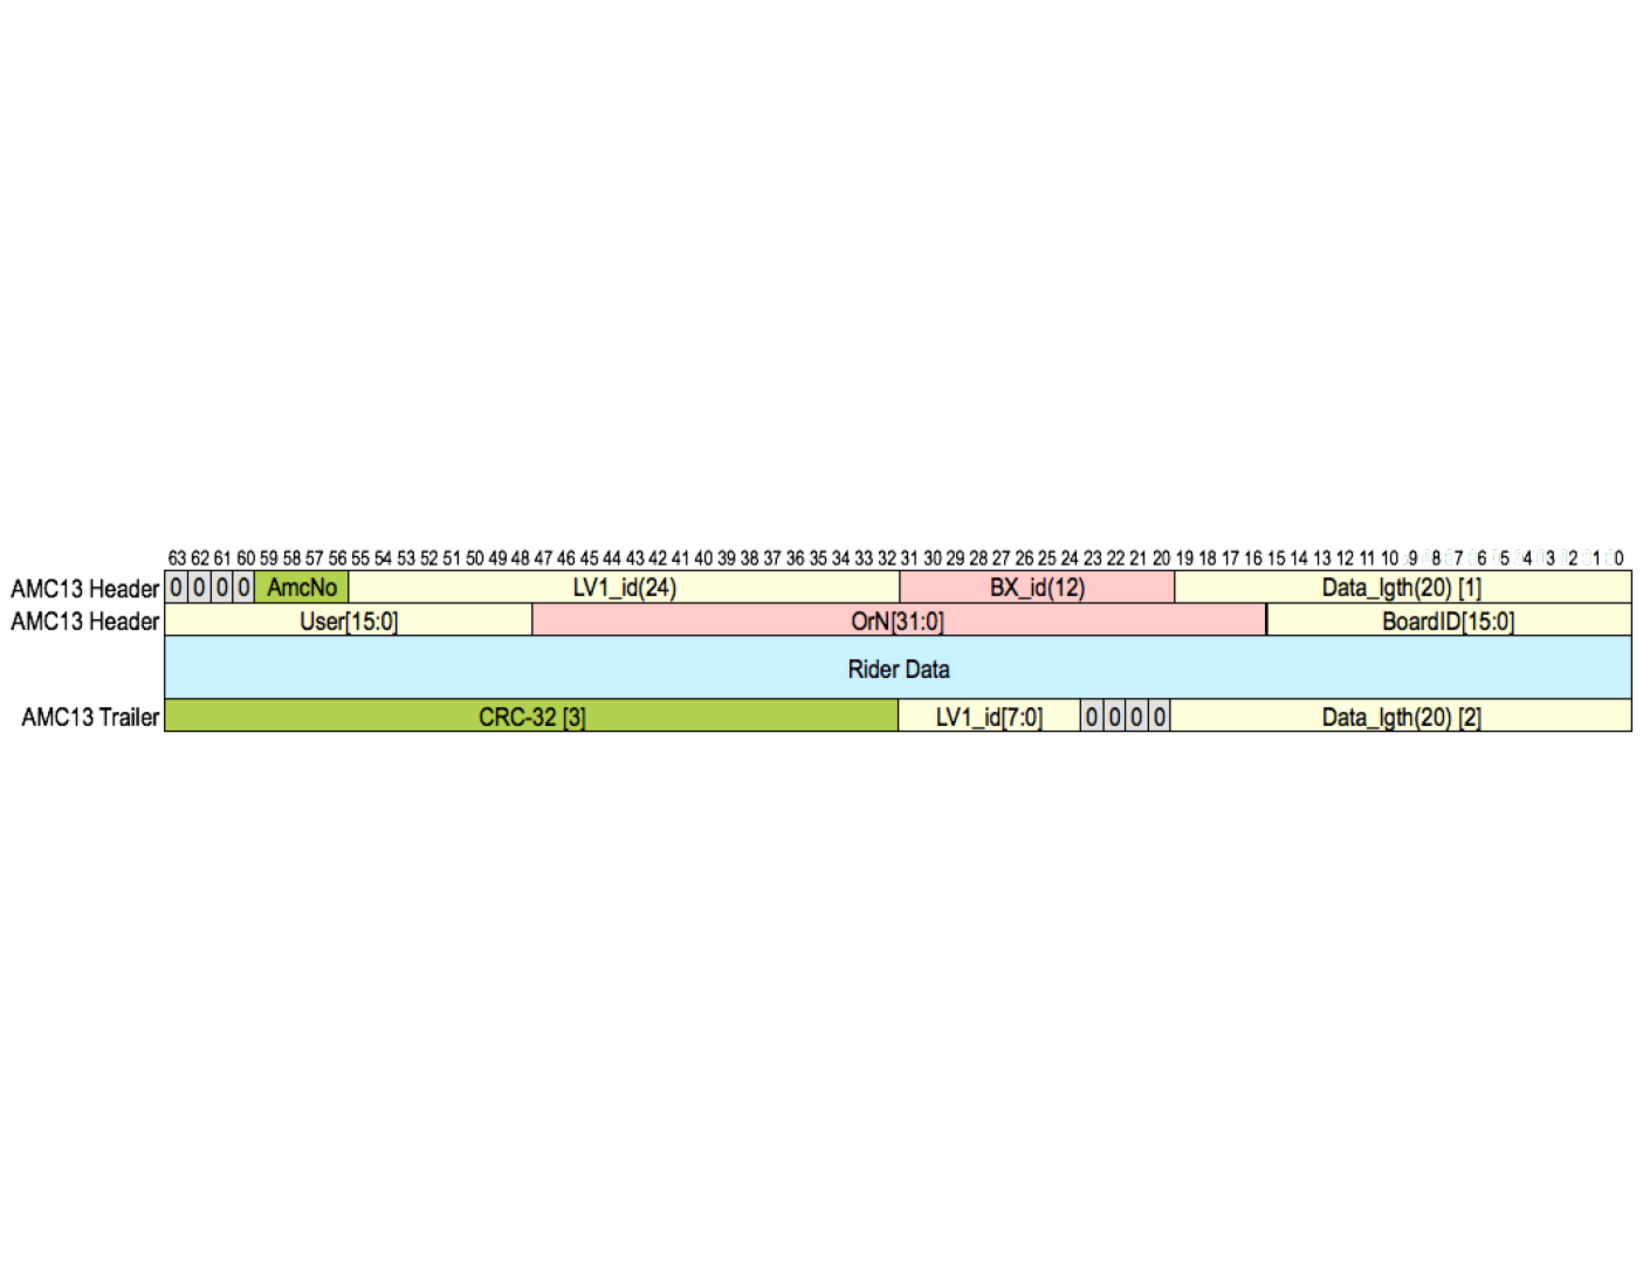
\includegraphics[trim=0cm 9.5cm 0cm 9.5cm ,width=0.95\textwidth]{pics/RiderToAMC13Header}
\caption{Rider to AMC13 data format.}
\end{figure}

%trim left bottom right top
\begin{figure}[htbp]
\centering
%\fbox{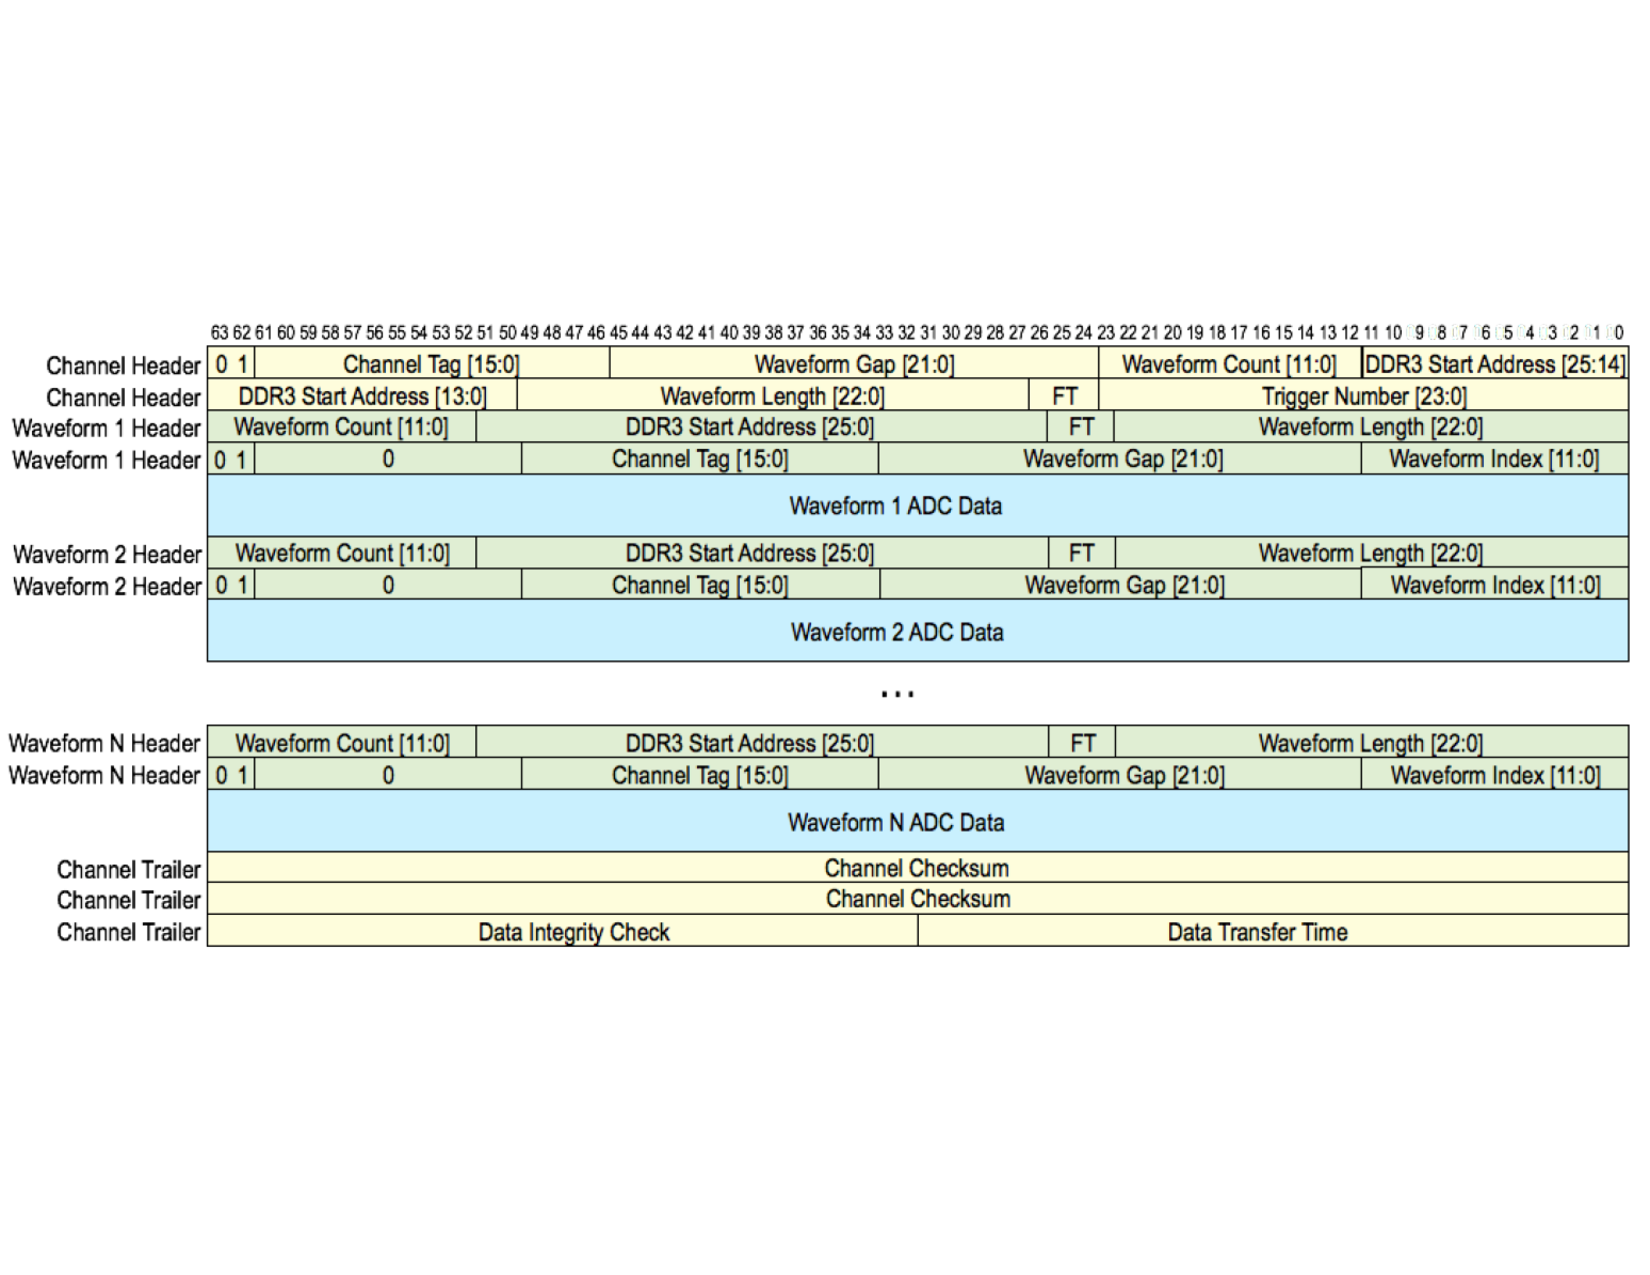
\includegraphics[trim=0cm 5.5cm 0cm 5.5cm ,width=0.9\textwidth]{pics/RiderChannelHeader}} guide line for trimming
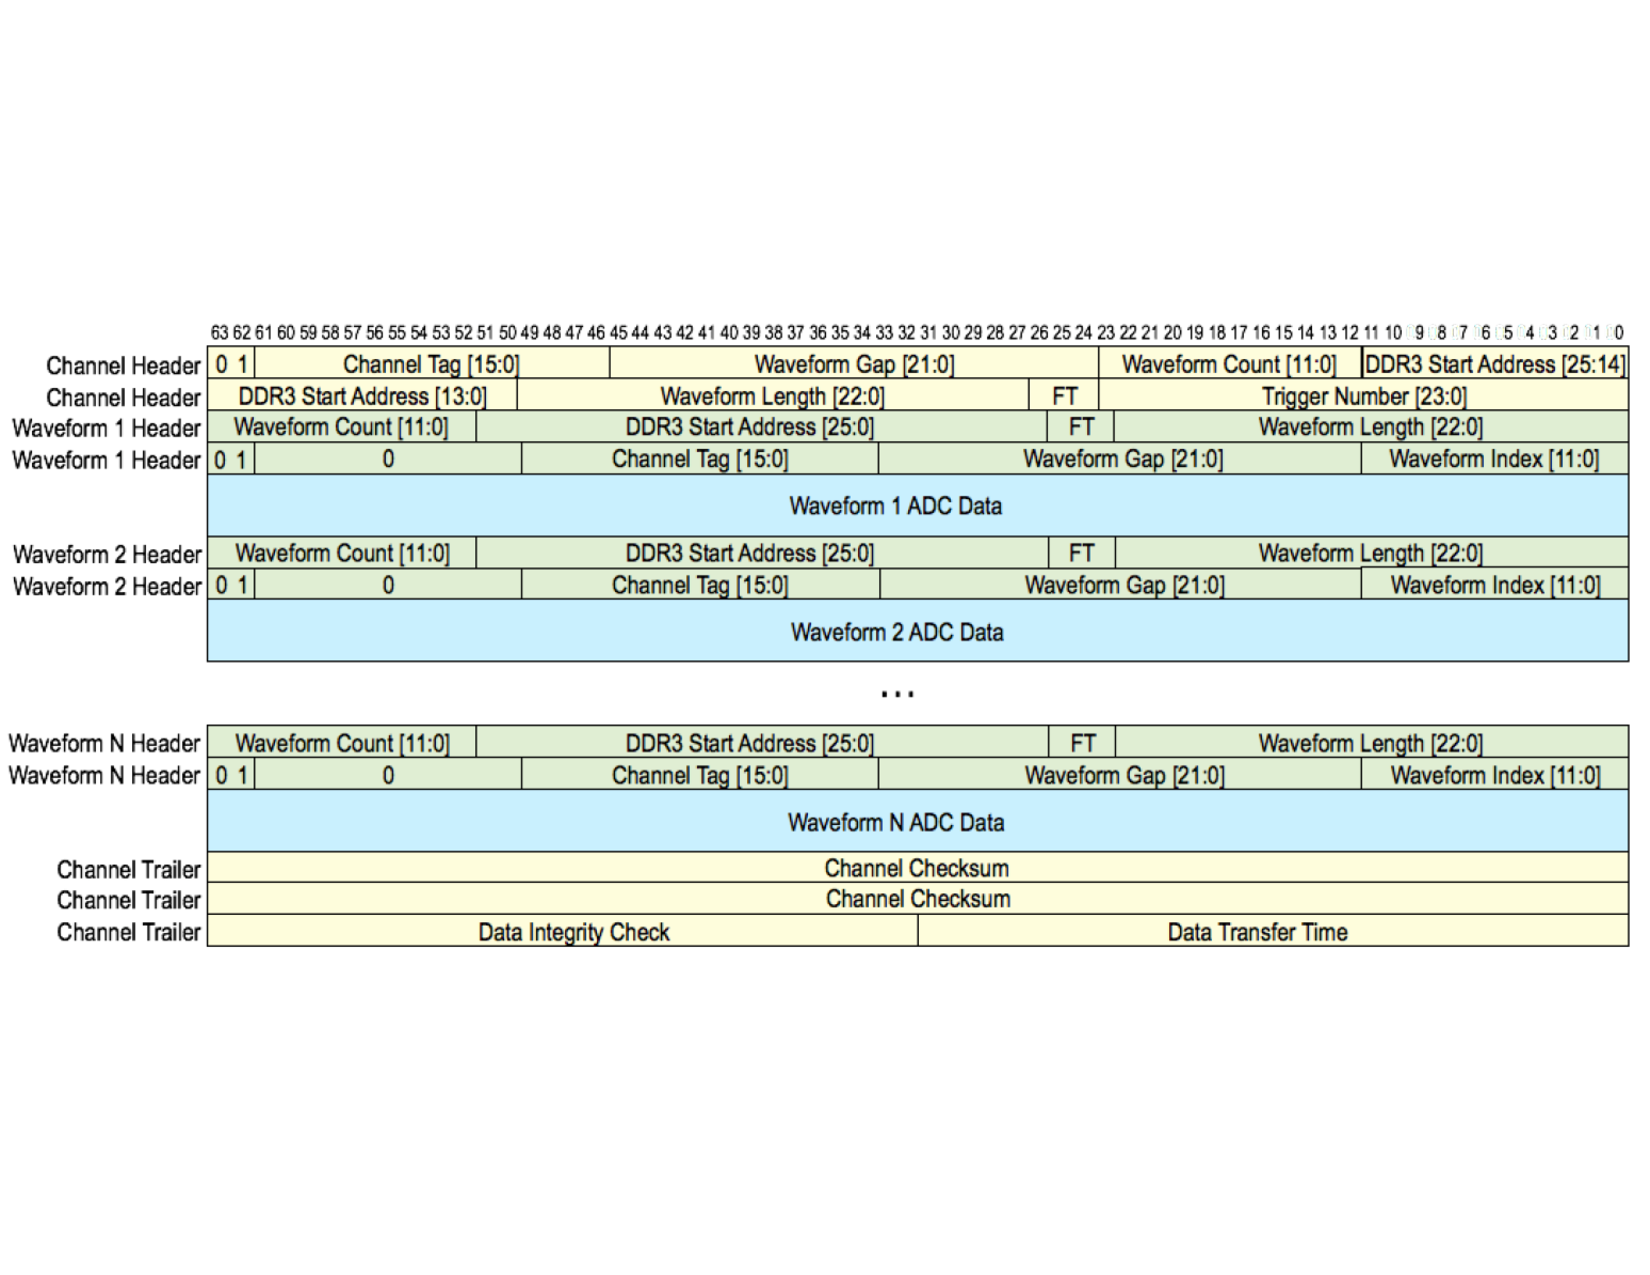
\includegraphics[trim=0cm 5.5cm 0cm 5.5cm ,width=0.95\textwidth]{pics/RiderChannelHeader}
\caption{Rider Channel data format.}
\end{figure}

\begin{figure}[htbp]
\centering
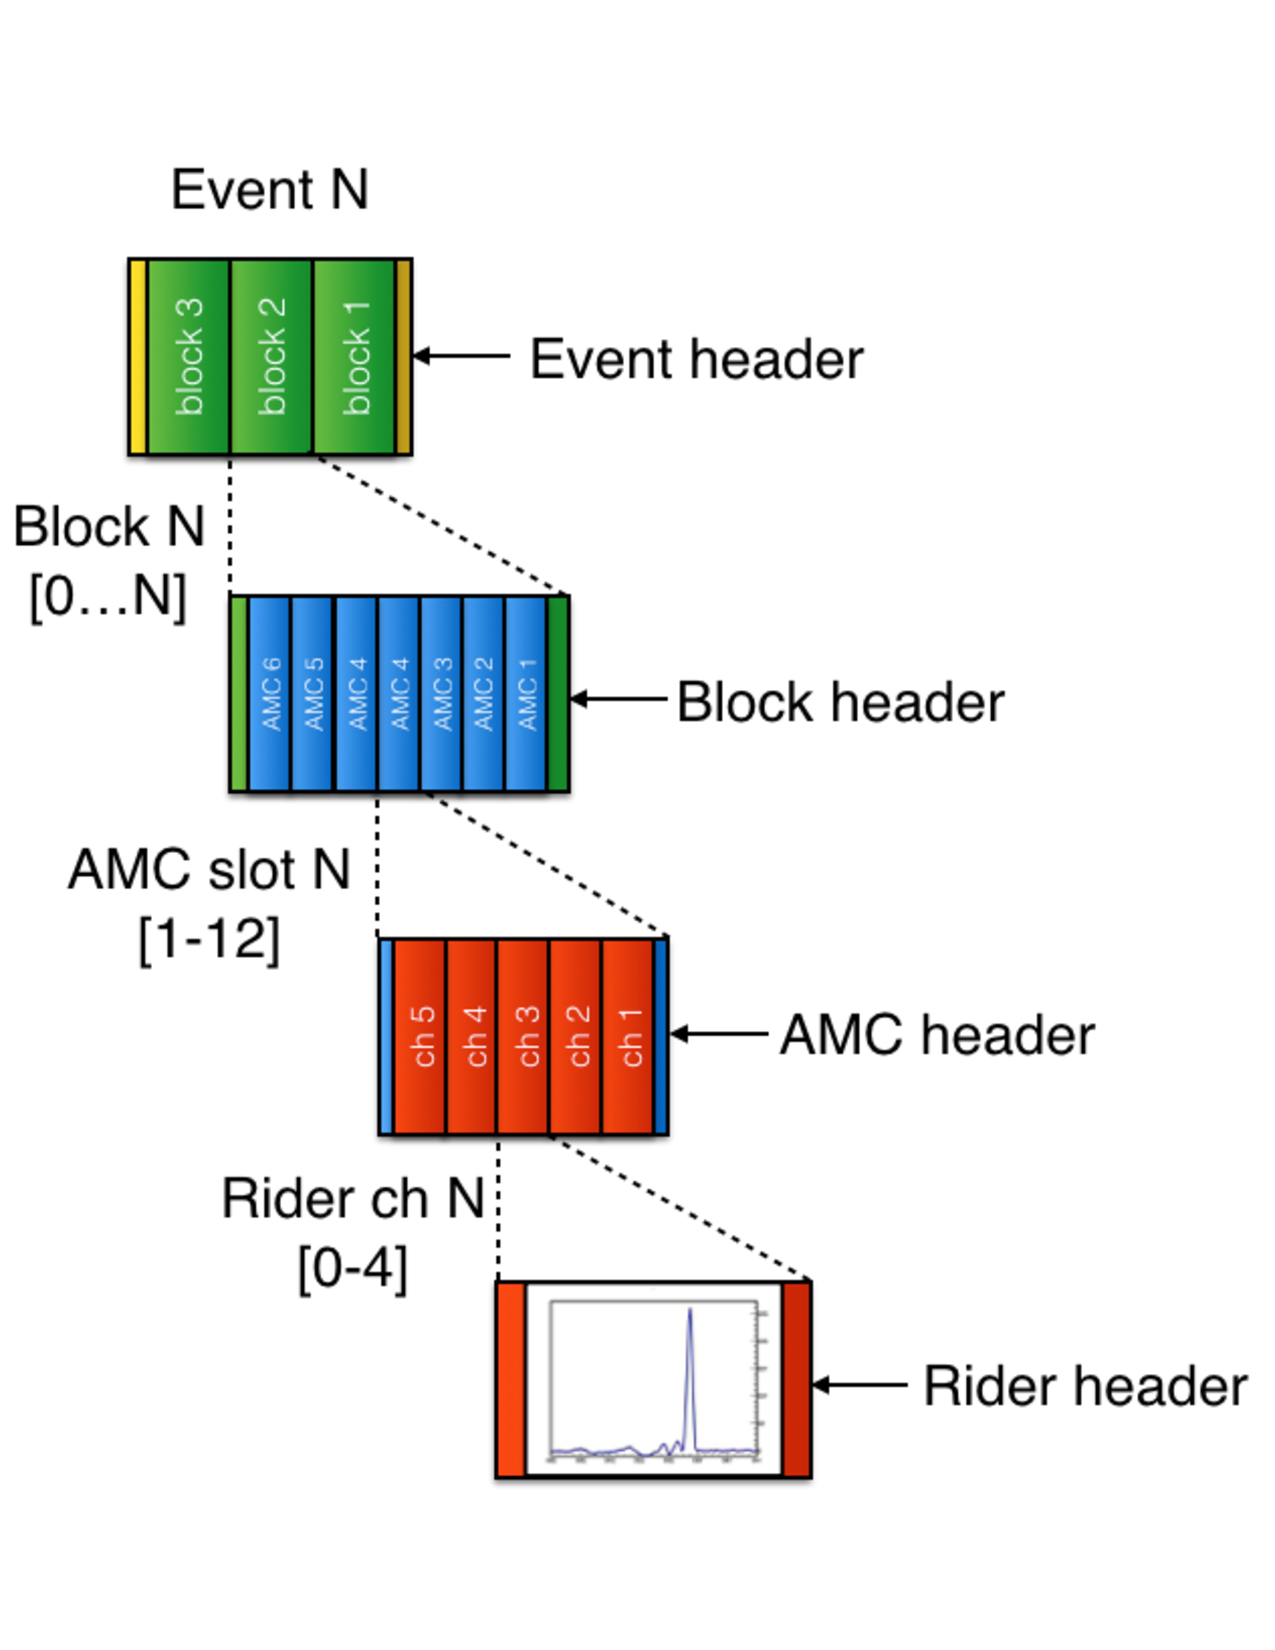
\includegraphics[width=0.9\textwidth]{pics/AllHeaders}
\caption{Per event data format}
\end{figure}


\newpage

\begin{thebibliography}{99}
\bibitem{Fienberg2015}
A. Fienberg et. al.,
\emph{Studies of an array of PbF$_{2}$ Cherenkvo crystals with large-area SiPM readout},
Nuclear Instruments and Methods in Physics Research Section A, Vol. 783, 12-21 (2015)

\bibitem{ROOT}
Rene Brun and Fons Rademakers, 
\emph{ROOT - An Object Oriented Data Analysis Framework},
Proceedings ALHENP'96 Workshop, Lausanne, Sep. 1996, Nucl. Inst. \& Meth. in Phys. Res. A 389 (1997) 81-86. See also \url{http://root.cern.ch}.

\bibitem{Khaw2016}
K. S. Khaw,
\emph{Offline structure group report},
FNAL E989 g-2 Experiment Document, FM2-doc-3781-v3 (2016). \url{http://gm2-docdb-fnal.gov:8080/cgi-bin/ShowDocument?docid=3781}

\bibitem{Midas}
TRIUMF MIDAS homepage, accessed May 13, 2016. 
\url{https://midas.triumf.ca/MidasWiki/index.php/Main_Page}

\end{thebibliography}

\end{document}

